\chapter{Conceptual Contributions}

\section{Overview of the Approach}

Our main goal is to elaborate a benchmark framework in order to systematically assess and analyze the performance of graph queries.

The well-known, state-of-the-art benchmark frameworks---such as BSBM, DBpedia and SP$^2$Bench---propose different, comprehensive use cases to measure the performance of graph queries over RDF data. BSBM and DBpedia uses such representative queries for the measurements that demonstrate the real-life use cases, and the SP$^2$Bench framework concentrates on the creation of various queries that mostly investigate the specific RDF data management approaches. As a conclusion, these frameworks guarantee a comprehensive performance evaluation of a workload---the ensemble of model, query and tool---by emphasizing the effect of the queries to the performance.

However, in the case of an arbitrary workload, the model also represents a dominating factor in the performance. Regarding the model, BSBM, DBpedia and SP$^2$Bench do not consider modifications in the model expect its size.

In order to introduce a new approach to the field of the well-known graph-based benchmark frameworks, we focus on elaborating a framework that proposes models with various characteristics, and investigates model and performance relationships of an arbitrary workload.

The main idea of our work and its possible utilization is depicted in Figure 1121212.%todo create overview optimization figure
In the first step, the framework analyzes the graph-based models and explores their characteristics, secondly, it evaluates the queries on the models and measures the performance---so the evaluation time. In the next step, the pairs of evaluation times and corresponding model characteristics are analyzed together, as the framework searches relationships between them. The goal is to find that how the characteristics of the models impact the performance of the queries.

As Figure 11212 %todo reference
illustrates as well, a possible utilization of our approach is the field of query optimization. Based on the analysis results from the framework, it becomes feasible to choose an appropriate optimization technique for a particular tool in the light of the model and performance relationship.

Three challenges can be found in our research. At first, we have to provide a solution for our framework to generate models with different characteristics that impact the performance of a certain query and thus cause a deviation in evaluation time. Secondly, we have to find model attributes that are able to characterize the models individually. Furthermore, these attributes must be suitable to create quantitative relationships among them and the evaluation times.

\section{Models and Metrics}
\subsection{Real-Life Networks}

In the discipline of graph theory, the internal structures of real-life networks are comprehensively investigated. The main approach in the analysis of these networks is to study the degree distributions of them and calculate some representative metrics---such as the clustering coefficient, average degree, average shortest path---that characterize the graphs appropriately. Based on the degree distributions and metrics, one can draw conclusion how a real-life network shows a similar characteristic to the well-known topologies such as the random graph, scale-free model, small-world model of Watts-Strogatz, and hierarchical network.

For example, the network of world-wide-web is studied in~\cite{www1} and ~\cite{www2}, and the authors notice that the degree distribution of the \textit{www} follows a power-law distribution with a heavy tail\footnote{Heavy tail means that there is a larger probability of receiving significantly higher values, than it is normally expected~\cite{heavy_tail}.}, which indicates the presence of web pages with a significantly higher degree (so a larger number of links) than the average degree. Though the probability of occurrences of these web pages is considerably lo, and thus, the connectivity of the world-wide-web can be represented by the scale-free model of Barabási and Albert.

%todo insert table from StatisticalMechanics_Rev of Modern Physics 74, 47 (2002)

More example can be found in the study~\cite{statistical_mechanics} of Barabási and Albert, as they review the advances of different publications and investigate the characteristics of different real-life networks. Empirical results prove that the \textit{movie actor collaboration network}, \textit{cellular networks}, \textit{phone call} and \textit{citation} networks also follow power-law distributions.
However, the small-world property and clustering coefficient metrics show significant fluctuations in these networks, which leads to the assumption that some of the investigated networks can be considered as scale-free models, however, some of them show small-world properties and high clustering similarly to the Watts-Strogatz or the hierarchical topology.

\subsection{Network Topologies and Representative Metrics}

The advances of the studies in real-life networks let us presume that the degree distributions and the consequent deviations in the model metrics are the foundations of our problem, namely, the generation of different models that are suited to impact the performance of graph evaluations.

In the same study~\cite{statistical_mechanics}, Barabási and Albert inspect the natures of various well-known graph topologies such as the random graph, scale-free and the Watts-Strogatz model. As a main result, they observe that there are significant differences among the topologies regarding specific graph metrics. For example, they show a considerable spread in the clustering coefficient and the average shortest path length per different graph topologies. 

Based on ~\cite{statistical_mechanics} and the research of hierarchical graphs~\cite{hierarchical}, the following metric deviations are assumed	between the four topologies, illustrated in Table \ref{tab:topology_metrics}. The random graph is considered as a reference point, and every value is compared to its metrics by assuming that the networks are in the same size.
\begin{table}[ht]
	\footnotesize
	\centering
	
	\begin{tabular}{ l c c c c}
		\toprule
		Metric & Random & Hierarchical & Scale-free & Watts-Strogatz \\ 
		\midrule 
		\textbf{Max Degree} & $\bullet$ & $\bullet \bullet \bullet$ & $\bullet \bullet \bullet$ & $\bullet$ \\ \hline
		\textbf{Clustering Coefficient} & $\bullet$ & $\bullet \bullet \bullet$ & $\bullet$ & $\bullet \bullet $\\ \hline
		\textbf{Average Shortest Path Length} & $\bullet$ & $\bullet \bullet$ & $\bullet$ & $\bullet \bullet$ \\ \hline
		\textbf{Degree Distribution} & Poisson & Power-law & Power-law & Uniform \\ \hline
		\bottomrule
	\end{tabular}
	\caption{Graph topologies and their descriptive metrics}
	\label{tab:topology_metrics}
\end{table}

As Table \ref{tab:topology_metrics} demonstrates, each topology can be characterized by different metric values, which leads to the assumption that if the diversity between the topologies may cause performance fluctuations of a particular query evaluation, then these metrics are adequate to characterize model and performance relationships quantitatively.

%todo use lattice ref in background
%todo emphasize lattice, random and p value in background, maybe add a picture as well

However, the values of metrics in Table \ref{tab:topology_metrics} are misleading due to two reasons. At first, the metrics of the Watt-Strogatz model highly depend on the initialization of the network, namely, the value of $p$ that is used in the generation\footnote{During the generation algorithm, every edge in the initial network is rewired with $p$ probability.}. The second problem connects to the max degree metric.  

At first, by modifying $p$, the Watts-Strogatz model represents a bridge between a lattice and a random graph. As Figure \ref{fig:ws} illustrates, the clustering coefficient ($C(p)$) and average shortest path ($L(p)$) metrics are changed with respect to $p$ scaling (figure in~\cite{ws_metrics}). The values are normalized by $L(0)$ and $C(0)$ that represent the clustering coefficient and average shortest path metrics for a lattice graph. As a conclusion, the Watts-Strogatz model shows significant deviations in these two metrics

\begin{figure}[!ht]
	\centering
	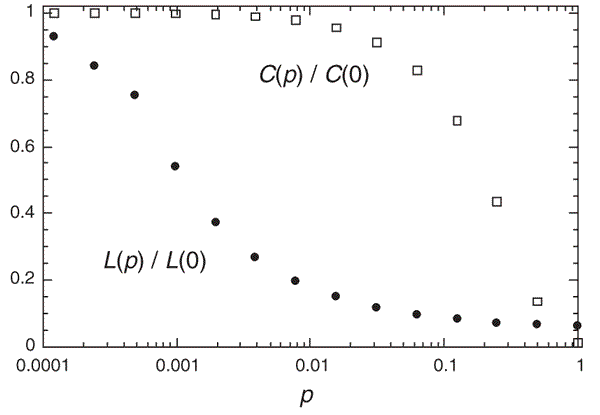
\includegraphics[width=130mm, keepaspectratio]{figures/ws_metrics.png}
	\caption{Characteristic path length L(p) and clustering coefficient C(p) of Watts-Strogatz model}
	\label{fig:ws}
\end{figure}

%todo add betweenness reference to background
The second problem relates to the maximum degree metric. This metric alone does not include a comprehensive information about the internal structure of the network. As a result, we introduce another metric, the \textit{betweenness centrality}, which is able to emphasize a higher degree's role in the graph, and thus, in the resulting query evaluation time.

After these minor modifications, the topologies and the related metrics are showed in the extended Table \ref{tab:topology_metrics2}.
\begin{table}[ht]
	\footnotesize
	\centering
	
	\begin{tabular}{ l c c c c c c}
		\toprule
		Metric & Random & Hierarchical & Scale-free & WS-0.1 & WS-0.01 & WS-0.001 \\ 
		\midrule 
		\textbf{Max Degree} & $\bullet$ & $\bullet \bullet \bullet$ & $\bullet \bullet \bullet$ & $\bullet$ & $\bullet$ & $\bullet$ \\ \hline
		\textbf{Clustering Coefficient} & $\bullet$ & $\bullet \bullet \bullet$ & $\bullet$ & $\bullet \bullet$ & $\bullet \bullet \bullet$ & $\bullet \bullet \bullet$\\ \hline
		\textbf{Average Shortest Path Length} & $\bullet$ & $\bullet \bullet$ & $\bullet$ & $\bullet $ & $\bullet \bullet$ & $\bullet \bullet \bullet$\\ \hline
		\textbf{Betweenness Centrality} & $\bullet$ & $\bullet \bullet \bullet$ & $\bullet \bullet$ & $\bullet$ & $\bullet$ & $\bullet$\\ \hline
		\bottomrule
	\end{tabular}
	\caption{Graph topologies and their descriptive metrics with extensions}
	\label{tab:topology_metrics2}
\end{table}


\subsection{Metric and Performance Comparison}

two algebraic connectivity

regression analysis

\subsubsection{Sample Choosing}

equal nodes and edges in samples, generation details not here

\section{Train Benchmark Framework}
use train for our approach
necessary extensions
1-2 paragraph
\section{Final Approach}

figure again with extensions


\subsection{Network Robustness and Metric Correlations}\label{sec:algebraic_connectivity}

Similarly,~\cite{algebraic1} and~\cite{algebraic2} investigate the random graph of Erdős-Rényi, the small-world graph of Watts-Strogatz and the scale-free graph of Barabási-Albert, however, the publishers also inspect the connectivity and robustness of the networks. In their case, a network is said to be robust if its performance is not sensitive to the changes in topology. In~\cite{algebraic1} the algebraic connectivity metric is studied in relation to graph’s robustness to node and link failures, however, they showed that the algebraic connectivity is not trivially correlated to the robustness of the network. The authors in~\cite{algebraic2} also drew the conclusion that there is no unique graph metric to satisfy both connectivity and robustness objectives while keeping a reasonable complexity, since each metric captures some attributes of the graph.



\subsection{Conclusions}

As the examples represent, there is a particular well-know subset of graph topologies that are widely analyzed. The random graph of Erdős-Rényi, the small-world model of Watts-Strogatz, and finally, a scale-free graph of Barabási-Albert. Moreover, numerous real-life networks show scale-free characteristics. We also investigate these networks topology, by reason of that they follow unlike degree distributions and they also show a variety in graph metrics. As far as metrics are concerned, we also give the assumption that the clustering coefficients and average path length metrics can characterize the model precisely, and thus, they can be considered as main indicators in the estimation of the query performance. Furthermore, we extend the set of observable metrics with the betwenness centrality as well.

Interesting and very important question is whether a unique metric is able to characterize a network's topology, and thus, more interestingly, whether it is suited to predict the performance of graph queries. As it was empirically determined in \ref{sec:algebraic_connectivity}, each metric captures some attributes of the graph, and only one is not adequate for the goal to characterize the network precisely. Besides the empirical results, we conjecture the same that only more than one, different metrics are suited to become appropriate performance estimators.


well-known topologies

What is main indicators in the models?

real-life networks + metrics
\section{Graph Topologies}

Random:
	The usage of a random graph in the framework is explained by the fact that its characteristic differs significantly from the other topologies, as it shows a Poisson degree distribution, and its descriptive metrics are smaller, especially the clustering coefficient, and betweenness metric. , indicating that for every pair of stations becomes adjacent by $p$ probability. 
	
WS:

	

\section{The Foundation of our Research}
use train benchmark, what is the limitations of it (already described the metamodel in related work)? what are the solutions? need analyzer components, a new model, new generation


\section{Uniform Model Generation}
only edges
\subsection{Calculate Edges in Hierarchical Network}

